% ------------------------------------------------------------------------------
% Palestra: Como os tradutores inativos do GNOME foram separados dos ativos
% Autores:
%     Adorilson Bezerra <adorilson@gmail.com>
% Licen�a Creative Commons Atribui��o 3.0. 
% Voc� pode usar e alterar este documento, 
% mas deve obrigatoriamente citar a autoria. 
% ------------------------------------------------------------------------------

\documentclass{beamer}

% ------------------------------------------------------------------------------
\usepackage[latin1]{inputenc}
\usepackage[brazil]{babel}
\usepackage{graphicx}
\usepackage{beamerthemesplit}
\usepackage{ae}
\usepackage{alltt}
\usepackage{pslatex}
% ------------------------------------------------------------------------------

\usecolortheme{beaver}

% ------------------------------------------------------------------------------
\title[Como os tradutores inativos do GNOME foram separados dos ativos]
{
    Como os tradutores inativos do GNOME foram separados dos ativos
}
\subtitle{Li��es aprendidas com hacking no Damned Lies}
\author[Adorilson Bezerra]
{
    Adorilson Bezerra
}
\date{\today}
\logo{
\includegraphics{img/gnome-gtp}}
% ------------------------------------------------------------------------------

\begin{document}

% ------------------------------------------------------------------------------
\frame{\titlepage}
% ------------------------------------------------------------------------------
\frame
{
    \frametitle{Ado... o que?}
    
\includegraphics[scale=0.3]{img/hackergotchi}
    \begin{itemize}
        \item adorilson @ internet
        \item adorilson.bezerra no ifrn.edu.br
    \end{itemize}
}

% ------------------------------------------------------------------------------
\section{Introdu��o}

%\subsection{Sobre o GNOME}

\subsection{Sobre o damned-lies}
\frame
{
    \frametitle{http://l10n.gnome.org}
    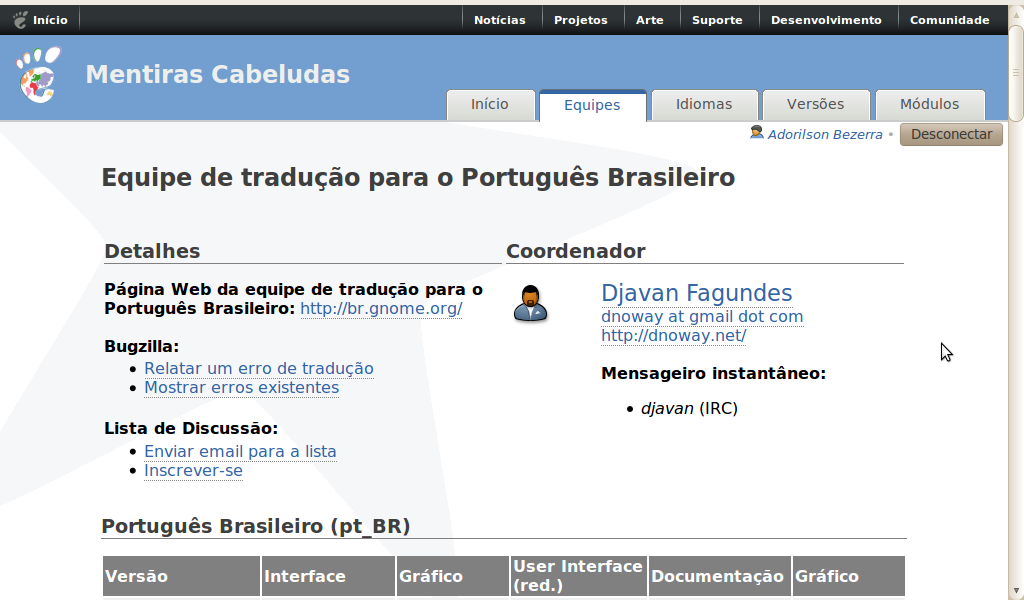
\includegraphics[scale=0.3]{img/dl}
}

\subsection{O Problema}
\frame
{
    \frametitle{Separar tradutores ativos e inativos}
    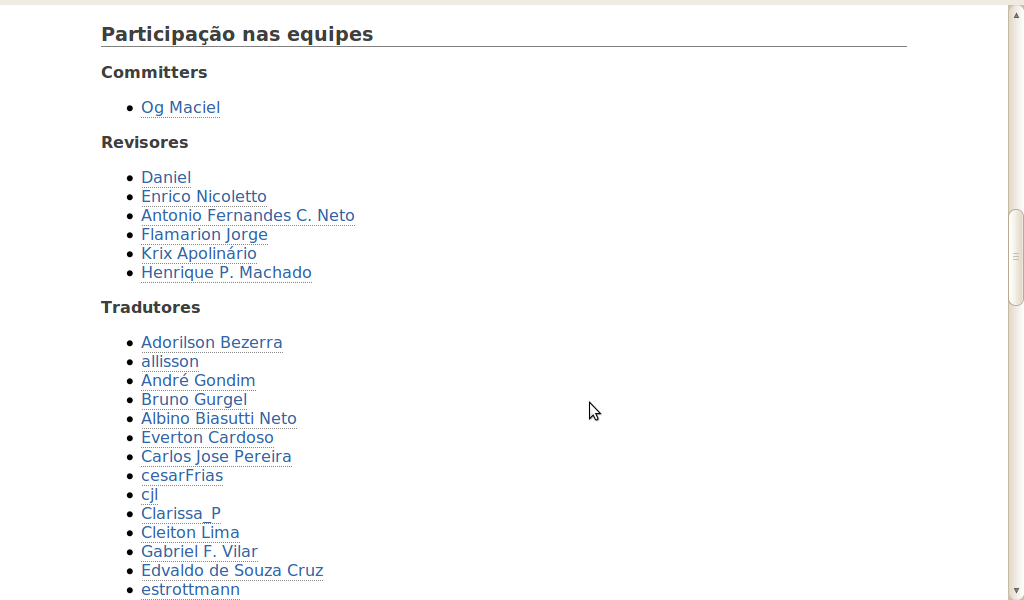
\includegraphics[scale=0.3]{img/dl2}
}

% ------------------------------------------------------------------------------
\subsection{O start}
\frame
{
    \frametitle{Eventos rocks!!!}
    \begin{figure}[t]
    \centering
        %http://blog.krix.com.br/2010/11/07/iv-ensl-e-vii-forum-gnome-%E2%80%93-parte-22/
        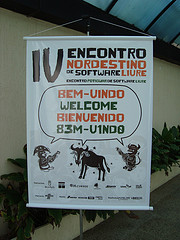
\includegraphics[width=3cm]{img/ensl}
        \hspace{0.1\textwidth}
        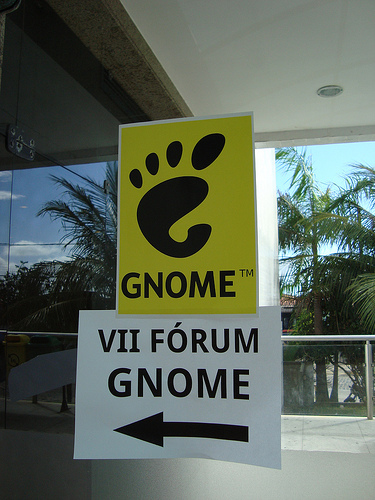
\includegraphics[width=3cm]{img/gnome1}
        \hspace{0.1\textwidth}
        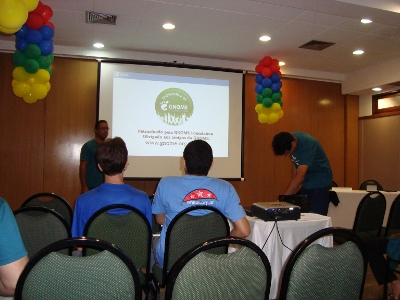
\includegraphics[width=3cm]{img/gnome2}
    \end{figure}
}
\frame
{
    \frametitle{Cria��o do bug em http://bugzilla.gnome.org => http://vai.la/2aqc}
    \begin{figure}[t]
        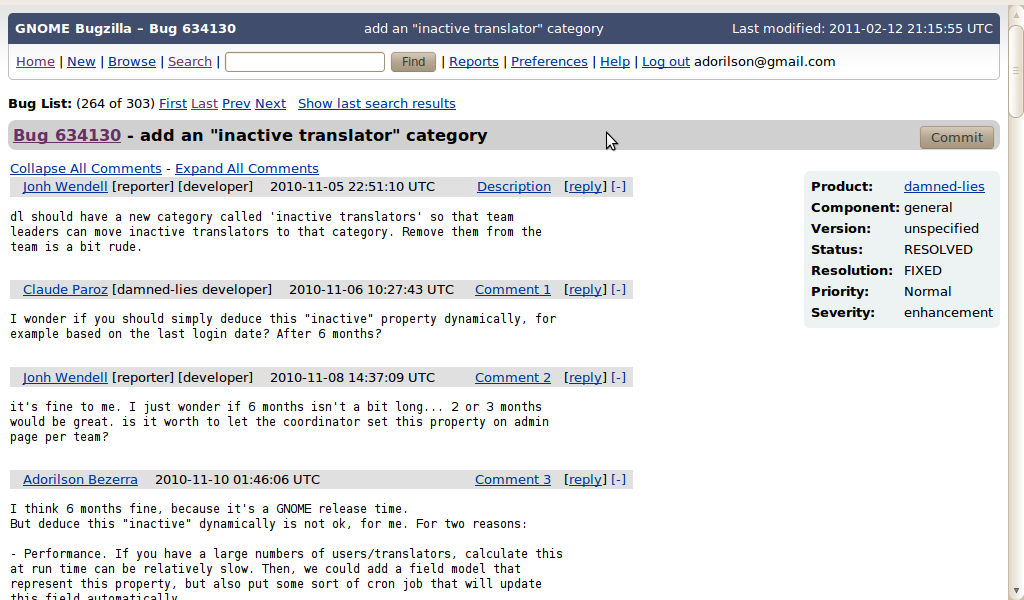
\includegraphics[scale=0.5]{img/bugzilla}
    \end{figure}
}

% ------------------------------------------------------------------------------

\section{Desenvolvimento}
\frame
{
    \frametitle{Du iu ispique inglishe?}
    \begin{figure}[t]
        
\includegraphics{img/flag_usa}
    \end{figure}
}
\frame
{
    \frametitle{Fa�a suas escolhas}
    \begin{figure}[t]
        
\includegraphics[scale=0.5]{img/python}
    \end{figure}
}
\frame
{
    \frametitle{IRC vive}
    \begin{figure}[t]
        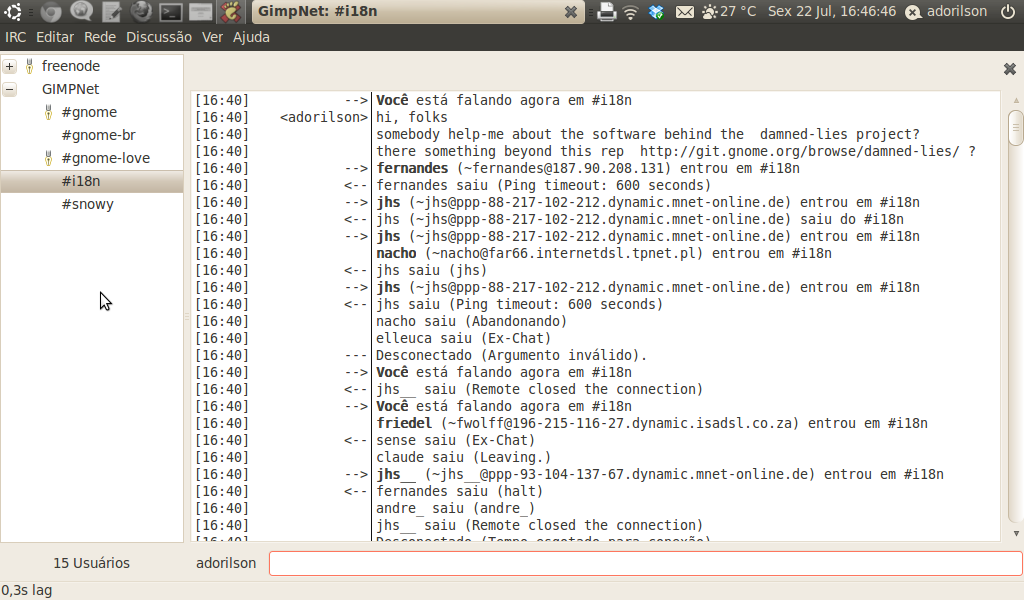
\includegraphics[scale=0.3]{img/irc}
    \end{figure}
}
\frame
{
    \frametitle{Discuta}
    \begin{figure}[t]
        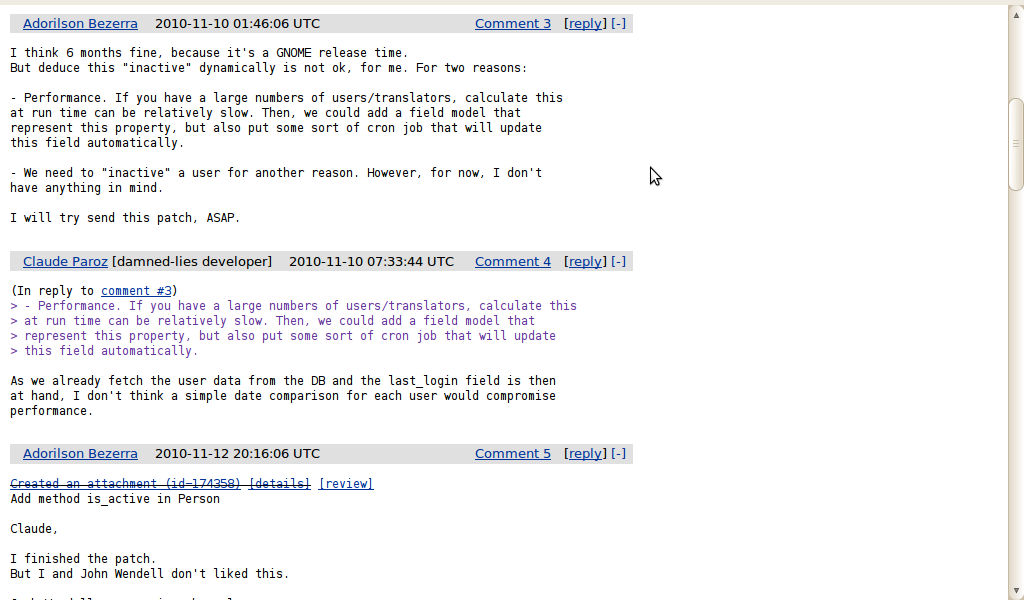
\includegraphics[scale=0.4]{img/discuta}
    \end{figure}    
}
\frame
{
    \frametitle{Show me the code}
    \begin{figure}[t]
        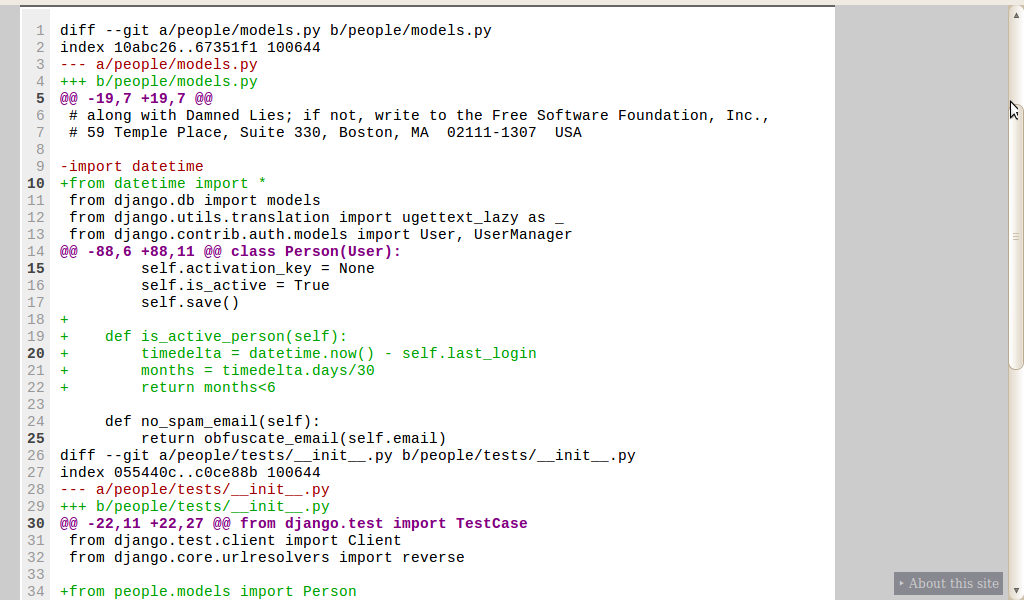
\includegraphics[scale=0.4]{img/patch1}
    \end{figure}
}
\frame
{
    \frametitle{Consiga um apoio}
    \begin{figure}[t]
        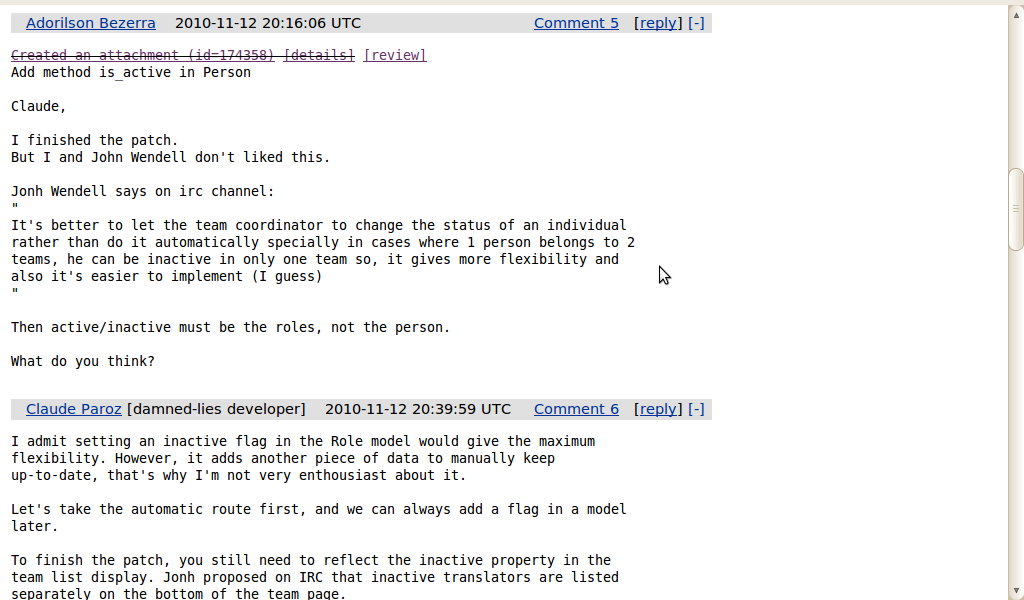
\includegraphics[scale=0.4]{img/mentor}
    \end{figure}
}
\frame
{
    \frametitle{Aprenda}
    \begin{figure}[t]
        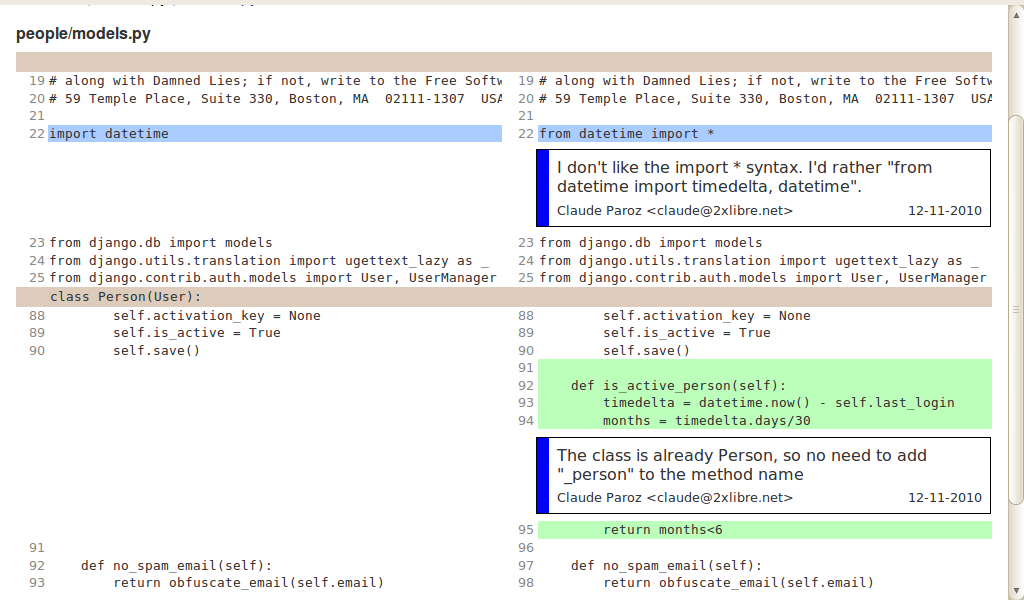
\includegraphics[scale=0.3]{img/aprenda}
    \end{figure}
}
\frame
{
    \frametitle{Cultive o desapego ao c�digo}
    \begin{figure}[t]
        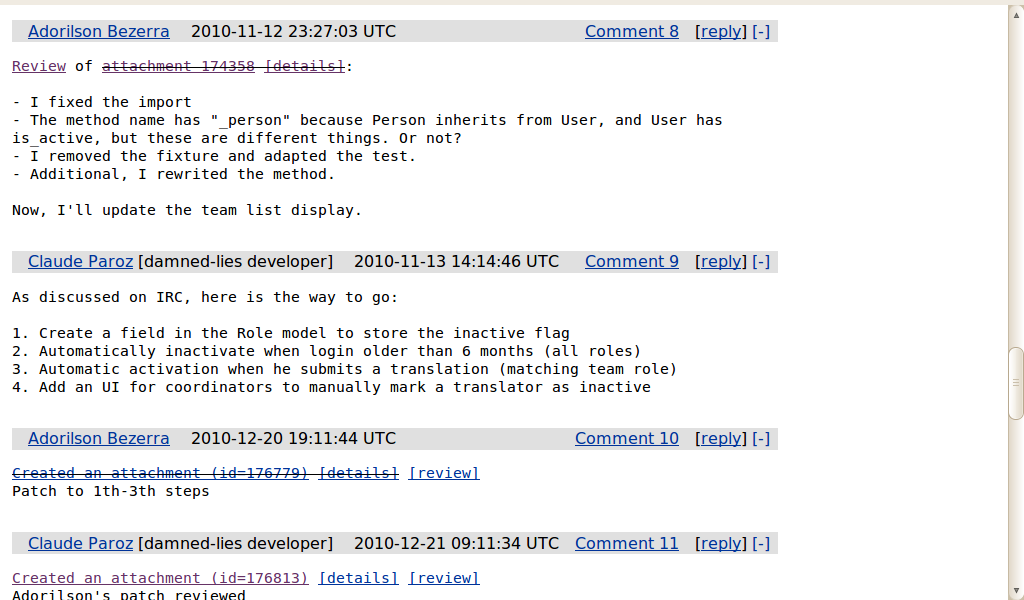
\includegraphics[scale=0.4]{img/desapego}
    \end{figure}
}
\frame
{
    \frametitle{Ao infinito e al�m}
    \begin{figure}[t]
        
\includegraphics[scale=0.7]{img/buzz}
    \end{figure}
}
\frame
{
    \frametitle{Ganhe o respeito}
    \begin{figure}[t]
        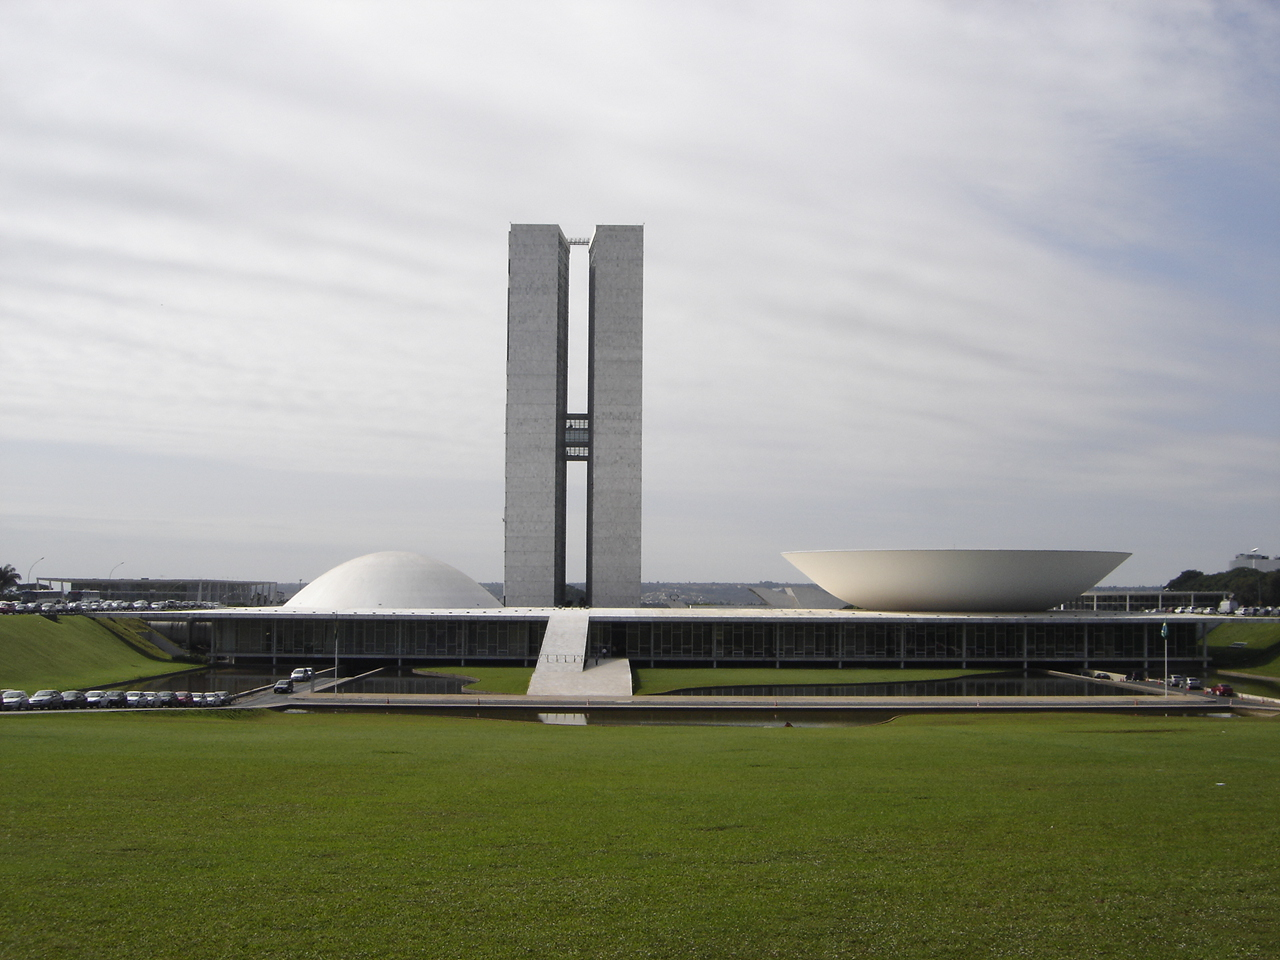
\includegraphics[scale=0.25]{img/brasilia}
    \end{figure}
}
\frame
{
    \frametitle{Espalhe}
    \begin{figure}[t]
        
\includegraphics[scale=0.5]{img/espalhe}
    \end{figure}
}

\section{Conclus�o}
\frame
{
    \frametitle{Software livre � bom para voc�}
    \begin{figure}[t]
        
\includegraphics[scale=0.6]{img/softwarelivre}
    \end{figure}
}


\end{document}
